% Źródła: materialy/2026-10-19/niezaleznosc.png i zdjęcia IMG_6950--IMG_6962.
\chapter{Niezależność}
\label{chap:niezaleznosc}

\poczatekwykladu{3}

\section{Niezależność dwóch zdarzeń}
\label{sec:niezaleznosc-dwoch}

Niech $(\Omega,\F,\PP)$ będzie przestrzenią probabilistyczną.

\begin{definicja}
\label{def:niezaleznosc-dwoch}
Zdarzenia $A,B\in\F$ są \emph{niezależne}, jeżeli
\begin{equation}
  \PP(A\cap B)=\PP(A)\PP(B).
  \label{eq:niezaleznosc-dwoch}
\end{equation}
\end{definicja}

\begin{uwaga}
Jeżeli $\PP(A)>0$ i zdarzenia $A,B$ są niezależne, to
\[
  \PP(B\mid A)=\frac{\PP(A\cap B)}{\PP(A)}
    =\frac{\PP(A)\PP(B)}{\PP(A)}=\PP(B).
\]
\end{uwaga}

\begin{przyklad}[Dwa rzuty kostką]
\label{przykl:kostka-niezaleznosc}
Rzucamy dwukrotnie uczciwą kostką; wyniki rzutów są niezależne.
Niech $A$ oznacza wyrzucenie szóstki w pierwszym rzucie,
$B$ wyrzucenie jedynki w drugim rzucie, a $C$ uzyskanie
parzystych wyników w obu rzutach. Sprawdźmy niezależność tych zdarzeń.
\end{przyklad}

\noindent\emph{Rozwiązanie.}
Przyjmujemy $\Omega=\{1,2,\ldots,6\}^2$ z jednakowo prawdopodobnymi
wynikami. Mamy
\[
  \PP(A)=\PP(B)=\frac16,
  \qquad \PP(C)=\frac12\cdot\frac12=\frac14.
\]
Ponadto
\begin{align*}
  \PP(A\cap B)&=\frac1{36}=\PP(A)\PP(B),\\
  \PP(A\cap C)&=\frac16\cdot\frac12=\frac1{12}
    \ne\frac1{24}=\PP(A)\PP(C),\\
  \PP(B\cap C)&=0\ne\frac1{24}=\PP(B)\PP(C).
\end{align*}
Zdarzenia $A$ i $B$ są niezależne, natomiast pary $A,C$ oraz $B,C$
nie są niezależne.

\begin{przyklad}[Rzuty monetą]
\label{przykl:moneta-niezaleznosc}
Rzucamy $n\geq2$ razy uczciwą monetą, niezależnie w kolejnych próbach.
Niech $A$ oznacza, że wypadła co najwyżej jedna reszka,
a $B$, że nie wypadły ani same orły, ani same reszki.
Dla jakich $n$ zdarzenia $A$ i $B$ są niezależne?
\end{przyklad}

\noindent\emph{Rozwiązanie.}
Wszystkie $2^n$ ciągów wyników są jednakowo prawdopodobne.
Zdarzenie $A$ obejmuje ciąg samych orłów oraz $n$ ciągów z jedną reszką,
więc
\[
  \PP(A)=\frac{1+n}{2^n},
  \qquad \PP(B)=1-\PP(B^c)=1-\frac2{2^n}.
\]
Dla $n\geq2$ zdarzenie $A\cap B$ oznacza dokładnie jedną reszkę,
stąd $\PP(A\cap B)=n/2^n$. Warunek niezależności jest równoważny
\begin{align*}
  \frac{n}{2^n}
    &=\frac{n+1}{2^n}\left(1-\frac2{2^n}\right),\\
  n2^n&=(n+1)(2^n-2),\\
  2(n+1)&=2^n,
  \qquad\text{czyli}\qquad n+1=2^{n-1}.
\end{align*}
Równość zachodzi dla $n=3$. Dla $n=2$ nie jest spełniona,
a dla $n\geq4$ mamy $2^{n-1}>n+1$ (nierówność utrzymuje się indukcyjnie).
Zatem \emph{zdarzenia są niezależne dokładnie dla $n=3$}.

\section{Niezależność rodzin zdarzeń}
\label{sec:niezaleznosc-rodzin}

\begin{definicja}
\label{def:niezaleznosc-rodziny}
Rodzina zdarzeń $(A_t)_{t\in T}$, gdzie $T$ jest dowolnym zbiorem indeksów,
jest \emph{niezależna}, jeżeli dla każdego $m\geq1$ i każdych parami różnych
$t_1,\ldots,t_m\in T$ zachodzi
\begin{equation}
  \PP\!\left(\bigcap_{i=1}^{m}A_{t_i}\right)
    =\prod_{i=1}^{m}\PP(A_{t_i}).
  \label{eq:niezaleznosc-rodziny}
\end{equation}
W szczególności zdarzenia $A_1,\ldots,A_n$ są niezależne, gdy
dla każdego $m\in\{2,\ldots,n\}$ i każdych indeksów
$1\leq t_1<\cdots<t_m\leq n$ spełniony jest wzór
\eqref{eq:niezaleznosc-rodziny}.
\end{definicja}

\begin{definicja}
\label{def:niezaleznosc-parami}
Zdarzenia $A_1,\ldots,A_n$ są \emph{parami niezależne}, jeżeli
\[
  \PP(A_i\cap A_j)=\PP(A_i)\PP(A_j)
  \qquad\text{dla wszystkich }i\ne j.
\]
\end{definicja}

\begin{definicja}
\label{def:dwie-rodziny}
Dwie rodziny zdarzeń $\mathcal{A},\mathcal{B}\subseteq\F$
są \emph{niezależne}, jeżeli dla każdych
$A\in\mathcal{A}$ oraz $B\in\mathcal{B}$ zachodzi
\[
  \PP(A\cap B)=\PP(A)\PP(B).
\]
\end{definicja}

\begin{definicja}
\label{def:rodzina-rodzin}
Rodziny zdarzeń $(\mathcal{A}_t)_{t\in T}$, gdzie
$\mathcal{A}_t\subseteq\F$, są \emph{niezależne}, jeżeli dla każdego
$m\geq1$, każdych parami różnych $t_1,\ldots,t_m\in T$ oraz dowolnych
zdarzeń $A_{t_i}\in\mathcal{A}_{t_i}$, $i=1,\ldots,m$, mamy
\[
  \PP(A_{t_1}\cap\cdots\cap A_{t_m})
    =\PP(A_{t_1})\cdots\PP(A_{t_m}).
\]
\end{definicja}

\begin{przyklad}[Niezależność parami nie wystarcza]
\label{przykl:niezaleznosc-parami}
Losujemy niezależnie i jednostajnie dwie liczby $x,y$ z odcinka $[0,1]$.
Przyjmujemy model geometryczny na $\Omega=[0,1]^2$ i zdarzenia
\begin{align*}
  A&=\{(x,y)\in\Omega:x\geq\tfrac12\},\\
  B&=\{(x,y)\in\Omega:y\geq\tfrac12\},\\
  C&=\{(x,y)\in\Omega:
    \min\{x,y\}>\tfrac12\ \text{lub}\ \max\{x,y\}\leq\tfrac12\}.
\end{align*}
Czy zdarzenia $A,B,C$ są niezależne?
\end{przyklad}

\noindent\emph{Rozwiązanie.}
Zdarzenie $C$ zajmuje dwa kwadraty leżące po przekątnej kwadratu
jednostkowego, jak na rysunku~\ref{fig:niezaleznosc-parami}.
Prawdopodobieństwa obliczamy jako pola odpowiednich obszarów:
\[
  \PP(A)=\PP(B)=\PP(C)=\frac12.
\]
Każde z przecięć dwóch zdarzeń ma pole $1/4$, zatem
\begin{align*}
  \PP(A\cap B)&=\frac14=\PP(A)\PP(B),\\
  \PP(A\cap C)&=\frac14=\PP(A)\PP(C),\\
  \PP(B\cap C)&=\frac14=\PP(B)\PP(C).
\end{align*}
Jednak
\[
  \PP(A\cap B\cap C)=\frac14
    \ne\frac18=\PP(A)\PP(B)\PP(C).
\]
Zdarzenia są więc parami niezależne, lecz rodzina $A,B,C$ nie jest niezależna.
Brzegi obszarów mają pole zero i nie wpływają na powyższe rachunki.

\begin{figure}[H]
  \centering
  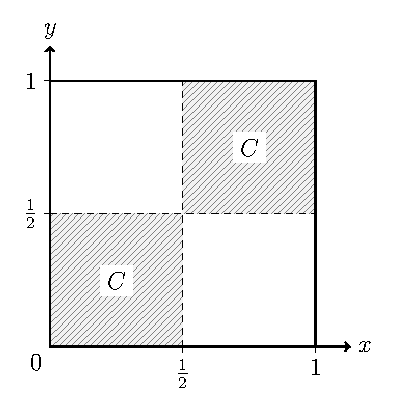
\includegraphics[width=6.5cm]{niezaleznosc-parami.pdf}
  \caption{Zdarzenie $C$ obejmuje dwa zakreskowane kwadraty.
    Zdarzeniu $A$ odpowiada prawa połowa, a $B$ górna połowa $\Omega$.}
  \label{fig:niezaleznosc-parami}
\end{figure}

\section{Własności niezależności}
\label{sec:wlasnosci-niezaleznosci}

\begin{fakt}
\label{fakt:wlasnosci-niezaleznosci}
Dla zdarzeń $A,B\in\F$ zachodzą następujące własności.
\begin{enumerate}
  \item Jeżeli $\PP(B)>0$ oraz $A,B$ są niezależne, to
    $\PP(A\mid B)=\PP(A)$.
  \item Jeżeli $A,B$ są niezależne, to niezależne są również pary
    $A,B^c$, $A^c,B$ oraz $A^c,B^c$.
  \item Jeżeli $\PP(A)=0$ lub $\PP(A)=1$, to $A$ jest niezależne
    od każdego zdarzenia $B\in\F$.
  \item Jeżeli $A$ jest niezależne od samego siebie, to
    $\PP(A)=0$ lub $\PP(A)=1$.
\end{enumerate}
\end{fakt}

\section{Schemat Bernoulliego}
\label{sec:bernoulli}

\begin{definicja}
\label{def:bernoulli}
\emph{Schematem Bernoulliego} nazywamy ciąg niezależnych powtórzeń
tego samego doświadczenia, w którym możliwe są tylko dwa wyniki:
\emph{sukces} z prawdopodobieństwem $p$ oraz \emph{porażka}
z prawdopodobieństwem $q=1-p$.
\end{definicja}

\begin{fakt}
\label{fakt:bernoulli}
W schemacie Bernoulliego prawdopodobieństwo uzyskania dokładnie $k$
sukcesów w $n$ próbach wynosi
\begin{equation}
  P_k=\binom{n}{k}p^k(1-p)^{n-k},
  \qquad k=0,1,\ldots,n.
  \label{eq:bernoulli}
\end{equation}
\end{fakt}

\begin{proof}
Przyjmujemy $\Omega=\{0,1\}^n$, gdzie $1$ oznacza sukces, a $0$ porażkę.
Dla $a=(a_1,\ldots,a_n)\in\Omega$ niezależność prób daje
\[
  \PP(\{a\})=p^{a_1+\cdots+a_n}(1-p)^{n-(a_1+\cdots+a_n)}.
\]
Zdarzenie uzyskania dokładnie $k$ sukcesów ma postać
\[
  A_k=\{(a_1,\ldots,a_n)\in\Omega:a_1+\cdots+a_n=k\}.
\]
Liczba takich ciągów wynosi $|A_k|=\binom nk$, a każdy z nich ma
prawdopodobieństwo $p^k(1-p)^{n-k}$. Zatem
\[
  \PP(A_k)=\binom nk p^k(1-p)^{n-k}.
\]
\end{proof}

\section{Granice ciągów zdarzeń}
\label{sec:granice-zdarzen}

\begin{definicja}
\label{def:granice-zdarzen}
Dla ciągu zdarzeń $(A_n)_{n\geq1}$ definiujemy \emph{granicę górną}
oraz \emph{granicę dolną} wzorami
\begin{align}
  \limsup_{n\to\infty}A_n
    &=\bigcap_{n=1}^{\infty}\bigcup_{k=n}^{\infty}A_k,
    \label{eq:limsup-zdarzen}\\
  \liminf_{n\to\infty}A_n
    &=\bigcup_{n=1}^{\infty}\bigcap_{k=n}^{\infty}A_k.
    \label{eq:liminf-zdarzen}
\end{align}
\end{definicja}

\begin{fakt}
\label{fakt:interpretacja-granic}
\leavevmode
\begin{enumerate}
  \item $\omega\in\limsup_{n\to\infty}A_n$ wtedy i tylko wtedy,
    gdy $\omega$ należy do nieskończenie wielu zdarzeń $A_n$.
  \item $\omega\in\liminf_{n\to\infty}A_n$ wtedy i tylko wtedy,
    gdy $\omega$ należy do wszystkich $A_n$ od pewnego indeksu,
    czyli do prawie wszystkich zdarzeń tego ciągu.
  \item $\displaystyle\liminf_{n\to\infty}A_n
    \subseteq\limsup_{n\to\infty}A_n$.
\end{enumerate}
\end{fakt}

\section{Lemat Borela--Cantellego}
\label{sec:borel-cantelli}

\begin{lemat}[Borela--Cantellego]
\label{lem:borel-cantelli}
Niech $(A_n)_{n\geq1}$ będzie ciągiem zdarzeń.
\begin{enumerate}
  \item Jeśli $\displaystyle\sum_{n=1}^{\infty}\PP(A_n)<\infty$, to
    \[
      \PP\!\left(\limsup_{n\to\infty}A_n\right)=0.
    \]
  \item Jeśli zdarzenia $A_n$ są niezależne i
    $\displaystyle\sum_{n=1}^{\infty}\PP(A_n)=\infty$, to
    \[
      \PP\!\left(\limsup_{n\to\infty}A_n\right)=1.
    \]
\end{enumerate}
\end{lemat}

\begin{proof}[Dowód punktu 1]
Oznaczmy $B_n=\bigcup_{k=n}^{\infty}A_k$. Ciąg $(B_n)$ jest malejący,
a jego przecięcie jest równe $\limsup_{n\to\infty}A_n$.
Z ciągłości prawdopodobieństwa dla ciągu malejącego
\eqref{eq:ciag-malejacy} oraz podaddytywności otrzymujemy
\begin{align*}
  0\leq\PP\!\left(\limsup_{n\to\infty}A_n\right)
    &=\lim_{n\to\infty}\PP(B_n)\\
    &=\lim_{n\to\infty}\PP\!\left(\bigcup_{k=n}^{\infty}A_k\right)\\
    &\leq\lim_{n\to\infty}\sum_{k=n}^{\infty}\PP(A_k)=0.
\end{align*}
Ostatnia granica jest zerowa, ponieważ są to ogony szeregu zbieżnego.
\end{proof}

\begin{proof}[Dowód punktu 2]
Ponownie korzystamy z ciągłości prawdopodobieństwa oraz z prawa de Morgana:
\begin{align*}
  \PP\!\left(\limsup_{n\to\infty}A_n\right)
    &=\lim_{n\to\infty}\PP\!\left(\bigcup_{k=n}^{\infty}A_k\right)\\
    &=1-\lim_{n\to\infty}\PP\!\left(\bigcap_{k=n}^{\infty}A_k^c\right)\\
    &=1-\lim_{n\to\infty}\lim_{N\to\infty}
      \PP\!\left(\bigcap_{k=n}^{N}A_k^c\right)\\
    &=1-\lim_{n\to\infty}\lim_{N\to\infty}
      \prod_{k=n}^{N}\bigl(1-\PP(A_k)\bigr).
\end{align*}
Ostatnia równość wynika z niezależności zdarzeń i ich dopełnień.
Z nierówności $1+x\leq e^x$, zastosowanej do $x=-\PP(A_k)$, dostajemy
\[
  0\leq\prod_{k=n}^{N}\bigl(1-\PP(A_k)\bigr)
    \leq\prod_{k=n}^{N}e^{-\PP(A_k)}
    =\exp\!\left(-\sum_{k=n}^{N}\PP(A_k)\right).
\]
Dla każdego ustalonego $n$ suma w wykładniku dąży do $+\infty$,
ponieważ $\sum_{k=1}^{\infty}\PP(A_k)=\infty$.
Stąd granica iloczynu przy $N\to\infty$ wynosi zero, a więc
\[
  1\geq\PP\!\left(\limsup_{n\to\infty}A_n\right)
    \geq1-\lim_{n\to\infty}
      \exp\!\left(-\sum_{k=n}^{\infty}\PP(A_k)\right)=1.
\]
To kończy dowód.
\end{proof}
